%\documentclass[12pt,a4paper,twoside]{book} 
\usepackage[spanish]{babel} % de pedro
\usepackage{graphics,graphicx,epsfig,color,float,afterpage,fancyheadings,subfigure,moreverb,alltt} % de pedro
\usepackage[latin1]{inputenc} % tildes de pedro

\usepackage{algorithm}
\usepackage{algorithmic}

\usepackage{rotating}
\usepackage{url}

%% Esta letra se convierte mejor a pdf que la normal
\usepackage{ae}

%%% Para las fuentes matemticas
\usepackage{amsfonts}

\usepackage{subfigure}

\usepackage{pstricks} % para los dibujos del da
\usepackage{lscape} % para las pginas en horizontal
\usepackage{portland} % para las pginas en horizontal
\usepackage{supertabular} % para las tablas de ms de una pgina
\usepackage{tabularx} % para las tablas del tipo tabularx
%\usepackage{glossary}
%\documentclass[a4paper,spanish,12pt]{book} % esto es de gustavo
%\usepackage{amsmath,amsfonts}   % underset mathbb
%\usepackage{authordate1-4}      % bib style
%\usepackage{epsfig}     % eps
\usepackage{epic}           % graficos
%\usepackage{eepic}           % graficos
\usepackage{curvesls}           % curvas
\usepackage{amssymb}
%\usepackage{fancyheadings}  % encabezados
%\usepackage{hhline}             % hhline
%\usepackage[latin1]{inputenc}   % tildes
%\usepackage{makeidx}        % ndices
%\usepackage{setspace}           % interlinea
%\usepackage[spanish]{babel} % espaol

%%%%%%%%%%%%%%%%%%%%%%%%%%%%%%%%%%%%%%%%%%%%%%%%%%%%%%%%%%%%%%%%%%%%%%%%%%%%%%%

\author{juanlu}
\title{Tesis de Juan Lus Jimnez Laredo}




\newcommand{\fecha}{\footnotesize{[ Impreso: \the\day-\ifcase\month\or
    Ene\or Feb\or Mar\or Abr\or May\or Jun\or Jul\or Ago\or Sep\or
      Oct\or Nov\or Dic\fi-\the\year ]}}

\newcommand{\N}{\mathbb{N}}

%% Para corregir las cabeceras largas
\newcommand{\cabecera}[2]{
\markright{\ref{#1}. \hspace{0.1ex} \MakeUppercase{#2}}}


%\pagestyle{headings}
%\renewcommand{\chaptermark}[1]{\markboth{\fecha \\ \\ #1}{}}
%\renewcommand{\sectionmark}[1]{\markright{#1 \\ \\ \fecha}}
%\addtolength{\headheight}{2.5pt}



%\lhead[\it\thechapter]{\sl\rightmark}
%\rhead[\rm\leftmark]{\it\thesection}
%\rfoot[]{\thepage}
%\cfoot[]{}
%\lfoot[\thepage]{}

%\thispagestyle{plain}

\setcounter{secnumdepth}{3}
\setcounter{tocdepth}{3}

%\renewcommand{\baselinestretch}{1.2}
%\setlength{\parskip}{0.8ex}

\newtheorem{theorem}{\sf Teorema}
\newtheorem{lemma}{\sf Lema}

\newcommand{\rem}[1]{\S\iffalse #1 \fi}
\newcommand{\cur}[1]{ {\it #1\/} }
\newcommand{\crcl}[1]{#1\kern-9pt\raise1pt\hbox{$\bigcirc$}}
\newcommand{\evag}{{\sf EvAg}}
\newcommand{\evagp}{{\sf EvAg.}}
\newcommand{\evags}{{\sf EvAgs}}
\newcommand{\evagsp}{{\sf EvAgs.}}

\newcommand{\prog}[2] {
   \small
   \begin{minipage}[t]{75mm} {\tt #1}  \end{minipage}
   \begin{minipage}[t]{60mm} {#2}      \end{minipage}
   \\
}
\newcommand{\prg}[2] { {\tt #1} & {\sf #2} \\}

\newcommand{\wmfspecial}[4]{
   \begin{figure}[h]
   \centerline{\psfig{figure=#1,height=#2}}
   \caption{#3}   \label{#4}
   \end{figure}
}                   % USO: \wmfspecial{nombre.eps}{altura}{leyenda}{etiqueta}

\def\stackunder#1#2{\mathrel{\mathop{#2}\limits_{#1}}}

\def\marco #1#2#3#4{\centerline{       % USO: \marco{.1}{10}{124mm}
  \vbox{\hrule height #1pt%
  \hbox{\vrule width #1pt\kern #2pt%
  \vbox{\kern #2pt%
  \vbox{\hsize #3\noindent #4}%
  \kern #2pt}%
  \kern #2pt\vrule width #1pt}%
  \hrule height0pt depth #1pt}} }


\newcommand{\symnote}[2]{\symbolnote{#1}{#2}}

\newfont{\bi}{cmbxti10 scaled\magstep1}       % bf + it


%% Ruta de las figuras
\graphicspath{{../figuras/}}


\begin{document}
           % Eliminarlo al compilar el documento maestro, ponerlo para compilarlo separado

%%%%%%%%%%%%%%%%%%%%%%%%%%%%%%%%%%%%%%%%%%%%%%%%%%%%%%%%%%%%%%%%%%%%%%%%%%%%%%%
%%                                                                           %%
%%                             Tesis Doctoral:                               %%
%%                         Juan Luis Jimenez Laredo                          %%
%%%%%%%%%%%%%%%%%%%%%%%%%%%%%%%%%%%%%%%%%%%%%%%%%%%%%%%%%%%%%%%%%%%%%%%%%%%%%%%

\cabecera{cap:methodology}{Experimental Methodology}
\chapter{\textit{Experimental Methodology}}
\label{cap:methodology}
\cabecera{cap:methodology}{Experimental Methodology}
%%%%%%%%%%%%%%%%%%%%%%%%%%%%%%%%%%%%%%%%%%%%%%%%%%%%%%%%%%%%%%%%%%%%%%%%%%%%%%%

%As exposed in the previous Chapter, the main motivation behind P2P EAs is tackling large instances in hard optimisation problems. To that aim, the {\em computational performance} of the EvAg model has been shown to succeed on demanding problems via massive scalability of P2P systems. Nevertheless, such results do not consider the {\em algorithmic performance} of the approach showing whether the algorithm is able to converge to convenient solutions or not, despite the asynchrony, nodes failures or dynamic changes on the population structure.

%As exposed at the Introduction of this thesis, the main motivation behind P2P EAs is tackling those large problem instances in which, due to memory or computational constraints, sequential approaches are unsuitable.

%With the aim of providing a framework to analyse the viability of P2P EAs, 

In the previous chapter we have presented the EvAg model as the framework with
which this thesis will analyse the viability of the P2P EC paradigm. In
addition, a first insight on the {\em computational performance} of the
approach has been provided showing that, for very demanding problems, it is able to scale following linear speedups. 

Nevertheless, such results do not take into account whether the
  algorithm is able to converge to convenient solutions in spite of the
  run-time dynamics of P2P systems. Hence, this chapter proposes an
%El capítulo no propone nada, lo haces tú - JJ
  experimental methodology for the analysis of the algorithm in a
  simulated P2P environment\footnote{ 
  All the source code for the experiments has been published under GPL
  v3 and is available from a
  Subversion repository at
  \url{https://forja.rediris.es/svn/geneura/evogen}. Accessed on March
  2010.} so that the viability of the P2P EA can be drawn from the {\em
  algorithmic performance} of the approach. % Es suficientemente
  % importante como para que no lo relegues a una nota 

Simulations will allow the execution of controlled experiments tackling
the goals exposed in Section \ref{sec:goals}. Section
\ref{sec:testcases} proposes a set of representative test-cases for
studying the viability of the model. In order to define the system with
a good level of detail, Section \ref{sec:decisions} describes the
decision-making process we have followed for the experimental
analysis. Finally and taking into account such decisions, Section
\ref{sec:overallmethodology} presents the overall methodology that will
be followed in the next chapter to tackle the different test-cases. 



 
%%%%%%%%%%%%%%%%%%%%%%%%%%%%%%%%%%%%%%%%%%%%%%%%%%%%%%%%%%%%%
\section{Goals}
\label{sec:goals}
%%%%%%%%%%%%%%%%%%%%%%%%%%%%%%%%%%%%%%%%%%%%%%%%%%%%%%%%%%%%%

As exposed at the introduction of this thesis, the main motivation behind P2P EAs is tackling those large problem instances in which, due to memory or computational constraints, sequential approaches are unsuitable. In this sense, analysing the scalability of the EvAg model is key to determine the approach viability. Additionally,
as the sizes of the problem instances increase, the number of computing nodes required to tackle the problem scales and, therefore, failures become more likely at run-time. Taking that into account, we propose an experimental analysis focusing on the following goals in order to prove the model viability:

\begin{enumerate}
\item Analysing the {\em scalability} of the model to demonstrate that the approach is suitable for tackling large problem instances in a failure-free environment.
\item Studying the {\em fault-tolerance} of the model under churn conditions to demonstrate that the model follows a {\em graceful degradation} and is able to tackle large problem instances in spite of churn.
\end{enumerate}


Studying the scalability makes possible not only  to analyse instances
under examination  % He cambiado esta frase, pero sigo sin
		   % entencerla. Será instance sizes?
but also forecasting the model behaviour in larger scenarios. On the other hand,  fault tolerance is a key issue in a P2P EA since churn is inherent to P2P systems given that peers are prone to failures.  

%%%%%%%%%%%%%%%%%%%%%%%%%%%%%%%%%%%%%%%%%%%%%%%%%%%%%%%%%%%%%
\section{Test-Cases}
\label{sec:testcases}
%%%%%%%%%%%%%%%%%%%%%%%%%%%%%%%%%%%%%%%%%%%%%%%%%%%%%%%%%%%%%

In order to tackle the previous goals, the following test-cases have been designed for the experimental analysis in the next chapter:

\begin{enumerate}
\item {\em Scalability of the model in failure-free environments against sequential approaches}. So that the EvAg model is compared against a canonical SSGA and a GGA to demonstrate that such a spatially-structured EA scales better than panmictic schemes of evolution.

\item {\em Influence of the population structure on the algorithm performance}. As explained in Section \ref{sec:evag}, there is no reason preventing the EvAg model to use population structures other than newscast. Therefore, this test-case aims analysing the scalability of the model using two common topologies in fine-grained approaches: a ring lattice \cite{giacobini:regular} and a Watts-Strogatz \cite{giacobini:evocop06} population structures (Figure \ref{fig:testcase2}). 

\begin{figure*}[htbp]
\centerline{\subfigure{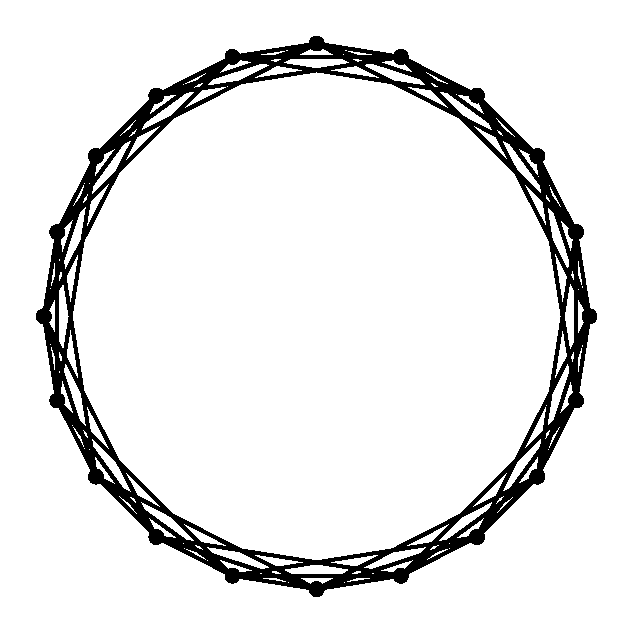
\includegraphics[width=1.5in]{WS-20-0000}
}
\hfil
\subfigure{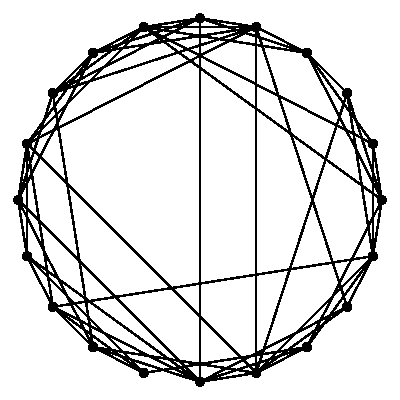
\includegraphics[width=1.5in]{WS-20-0200}
}
\hfil
\subfigure{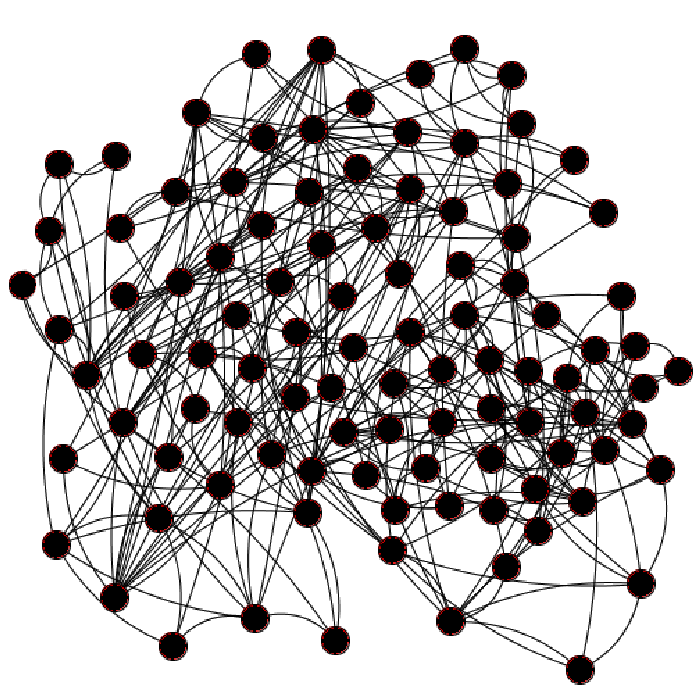
\includegraphics[width=1.5in]{newscastgraph}
}}
\caption{ From left to right: ring, Watts-Strogatz and newscast population structures.
}
\label{fig:testcase2}
\end{figure*}

\item {\em Fault tolerance of the model}. In this test-case, we will analyse the scalability of the model using several scenarios of churn in which the system degrades under different failure rates.


\end{enumerate}



%%%%%%%%%%%%%%%%%%%%%%%%%%%%%%%%%%%%%%%%%%%%%%%%%%%%%%%%%%%%%
\section{Decisions on the experimental analysis}
\label{sec:decisions}
%%%%%%%%%%%%%%%%%%%%%%%%%%%%%%%%%%%%%%%%%%%%%%%%%%%%%%%%%%%%%

Given the huge complexity of either P2P systems or EAs, a detailed
analysis on their interactions in the P2P EC paradigm remains  % o lays
				% - JJ
 beyond the scope of this thesis. Hence, a certain number of decisions has to be made in order to focus the analysis on the specifications of the goals. Therefore, this Section aims to justify the simplifications and assumptions made on the model.


\subsection{Simplifications}

% No tengas comienzos vacíos. Por ejemplo, la última frase de la
% introducción podías ponerla aquí - JJ

\begin{itemize}
   \item The experimental analysis in this thesis will concentrate on {\em binary-coded GAs} \cite{eiben:eas} within the rest of EC paradigms such as ES \cite{es:rechenberg}, EP \cite{ep:fogel} or GP \cite{gp:koza}. The main reason is that the population sizing theory \cite{goldberg:competent} that we will follow to perform analysis on the scalability of the algorithm focuses on such kind of EAs.  Nevertheless, taking into account that {\em binary-coded GAs} follow the same evolutionary scheme than other EAs such as {\em real-coded GAs} \cite{rcga:eshelman} or GP, conclusions should be easily extended to other paradigms.
   
   \item With the aim of establishing a worst-case analysis,
	 evolutionary operators will not apply specific knowledge on the
	 problem. In this sense, we will use  {\em uniform crossover},
	 {\em bit-flip mutation} as operators and {\em binary
	 tournament} as decentralised selection mechanism throughout all
	 the experiments \cite{eiben:eas}. Either {\em uniform
	 crossover} or {\em bit-flip mutation} prevent the algorithm
	 search to form higher order BBs, thus challenging the GA's
	 search mechanisms. % esto no acabo de creérmelo, así que
	 % tendrías que justificarlo. Los higher-order BBs pueden
	 % crearse por selección, y si los mendas son muy parecidos, se
	 % preservan con el uxover - JJ

   \item In the same line than the previous point, individuals will be {\em initialised at random}. Every gene will have an uniform probability of $0.5$ to be either $1$ or $0$, so that, on average, the randomly generated initial population is placed on local optimum attracting regions for the problem landscapes proposed in Section \ref{sec:benchmark}.
   
\end{itemize}

\subsection{Assumptions}

% Igual aquí. Mete algo.  - JJ

\begin{itemize}
   
   \item We have used selectorecombinative versions of the algorithms
	 (without mutation) for estimating the population sizes. Lobo
	 and Lima state in \cite{lobo07:review} that the assumption of a
	 selectorecombinative GA is commonly made in population sizing
	 studies as the only source of diversity is then the initial
	 population which stands for a worst case analysis. However,
	 this thesis complements the study analysing the convergence of
	 the approach using mutation. 
   
    \item We assume that every EvAg behaves as a {\em virtual node}
	  \cite{dynamo:virtualnodes} in such a way that every physical
	  node can host more than a single EvAg. Hence, the number of
	  {\em virtual nodes} hosted in a physical one can be decided at
	  a load-balance level depending on node capacities and a
	  heterogeneous system such as P2P can be assumed as homogeneous
	  at a virtual level. 
   
   \item Despite having assumed homogeneous conditions in the previous
	 point, the lack of a central clock in a decentralised scheme
	 implies an asynchronous execution. In this sense, the most
	 commonly used methods to simulate asynchrony either in cellular
	 automaton \cite{asynchrony:ca} or cellular evolutionary
	 algorithms \cite{tomassini} are: 
   
   \begin{itemize}
   \item {\em Fixed line sweep}, the idea here is that the update on the different cells (i.e. EvAg in our case) follows a prestablished sequential order, e.g. from left to right in rings structured populations.
   \item {\em Fixed random sweep}, it consists in a small variation on the previous method in which the update sequence is set randomly at the beginning of a run as a permutation of the different cells.
   \item {\em New random sweep}, a new random cell permutation is generated at every cycle of a run, understanding a cycle (or time step) as the sequential update of all the cells. 
   \item {\em Uniform choice}, the next cell to be updated is randomly chosen with uniform probability from all the possible cells. This method implies that the same cell could be updated more than once during a cycle and, in turn, some others could remain without updating.
   \end{itemize}
   
% No me parece que lo de arriba venga muy a cuento. Sería mejor que
	 % dijeras que has elegido uniform, y que hay otros tipos que no
	 % te vienen bien porque requieren una secuencia. La morralla,
	 % cuando menos mejor - JJ 
To the choice of an adequate update policy for our approach,  the {\em uniform choice} policy seems more appropriate to model a decentralised run in which there is no guarantee of any sequential order in the update of the individuals. This way, we have adopted such a policy to simulate the asynchronous update of $EvAgs$.

In addition, it has to be considered that Dorronsoro et al. show in
	 \cite{dorronsoro:asynchrony} that the four methods do not
	 almost %always? - JJ
 present statistical differences between each other in a test-suite of 4
	 % no uses números en el texto, usa la palabra. - JJ
 different problems. The uniform choice method presents statistical
	 differences from the rest in a single case, indicating that
	 choosing between these methods does not have a great influence
	 on the algorithm performance. 

   \item Every time that an $EvAg$ % si usas esto, úsalo siempre, pero
	 % yo creo que es mejor que definieras una macro \evag y que
	 % fuera, por ejemplo, {\sf EvAg} - JJ
performs a fitness evaluation, it also initiates a cache exchange of the
	 newscast protocol, i.e. $t_r=cycle$ where $t_r$ is the
	 parameter for the newscast updating frequency exposed in
	 Section \ref{sec:p2pnewscast} and {\em cycle} is defined as the
	 time the algorithm takes to perform $n$ evaluations in a
	 population of $n$ $EvAgs$ using {\em uniform choice}.
   
   \item The evolutionary algorithm  will begin at $t_r=20$ to guarantee that the newscast protocol bootstraps and converges given that it has already shown in Section \ref{sec:bootstrapping} that the protocol takes at around 12 cycles to converge to an state of dynamic equilibrium for a network size of $1600$. In this sense, we have assumed a synchronised start up of the experiments. 

  \item The cache size ($c$) is the only tunable parameter in newscast and we use $c=20$ within all the settings of the experiments. Such value takes into account Jelasity and van Steen recommendations in \cite{jelasity:newscast} stating that the intended normal setting of newscast is $c \ll n$ and demonstrating that values from $c=20$ prevent the spontaneous partitioning of the graph even when it becomes very large (see Section \ref{sec:newscastrobustness} for more details). In addition, we make experiments for the fine-tuning of the parameter in the appendix of this thesis showing a lack of influence of $c$ on the EvAg performance when $c \in [0.005n,0.15n]$, where $n$ is the population size.

 \item We have assumed that the time required for communications is
       negligible. Such an assumption might be unrealistic for
       small problem instances, but it turns feasible for problem instances
       becoming large, as it has been shown in the analysis of the
       parallel performance of the model in Section
       \ref{sec:parallelperformance}.  % How large? A partir de cuánto
       % no tiene importancia? Esto no creo que sea cierto, pero
       % bueno... tienes que justificarlo mejor - JJ

 
\end{itemize}

% Ninguna conclusión o sumario - JJ





%%%%%%%%%%%%%%%%%%%%%%%%%%%%%%%%%%%%%%%%%%%%%%%%%%%%%%%%%%%%%
\section{Methodology}
\label{sec:overallmethodology}
%%%%%%%%%%%%%%%%%%%%%%%%%%%%%%%%%%%%%%%%%%%%%%%%%%%%%%%%%%%%%

%This thesis analyses the scalability of the EvAg model from the perspective of the population sizing theory \cite{gwoldberg:competent}  which states that there is an optimal criterion for tuning the population size of an EA for a given problem instance and difficulty. Within this thesis, the population size has been empirically estimated using the method explained in Section \ref{sec:bisection} that tunes the minimum population size $N$ required to supply enough building blocks (BBs) so that a selectorecombinative Genetic Algorithm (GA) will converge toward optimal solutions. The assumption of a selectorecombinative GA (without mutation) is commonly made in population sizing studies as the only source of diversity is then the initial supply of raw BBs which stands for a worst case analysis \cite{lobo07:review}.


In order to analyse the scalability of the EvAg model, experiments are
conducted on trap functions (described in Section
\ref{sec:benchmark}). %Incluye hyperref, creo, para que genere
		      %hiperenlaces internos automáticamente
 The purpose is investigating how population sizes scale with increasing problem size and difficulty. To this end, we follow the population sizing theory \cite{goldberg:competent} which states that there is an optimal population size for a given problem instance that can be determined under some conditions. In particular, we use the bisection method (Section \ref{sec:bisection}) that determines the minimum population size $N$ for a selectorecombinative GA, i.e., a GA without mutation. 
%The assumption of a selectorecombinative GA is commonly made in population sizing studies as the only source of diversity is then the initial population which stands for a worst case analysis \cite{lobo07:review}. 
In addition, we look at the scale-up properties of the average number of evaluations to a solution (AES), which is a device independent measure of computational effort that can be used for all EAs, with or without mutation \cite{eiben:eas}. Finally, the study is complemented switching mutation on, so that, the algorithm convergence is analysed for the most demanding problem instances using the metrics proposed in Section \ref{sec:metrics}. Such results will be statistically analysed using the non-parametric Wilcoxon test.




\subsection{Test-suite}
\label{sec:benchmark}
%%%%%%%%%%%%%%%%%%%%%%%%%%%%%%%%%%%%%%%%%%%%%%%%%%%%%%%%%%%%%

%No está bien comenzar con un gerundio, porque necesitas varias líneas
%para saber qué es lo qeu estás haciendo siguiendo a Lobo y Lima. Di que
%haces, y luego por qué - JJ
% Modificado! - Juanlu
Experiments were conducted on deceptive, quasi-deceptive, and non-deceptive trap functions \cite{ackley:trap}
following Lobo and Lima's recommendations in \cite{lobo07:review} about choosing a test suite with known population requirements and investigating the scalability on landscapes with different characteristics.  These functions represent a set of decomposable problems based on unitation and composed of ($m$) sub-functions in which the total fitness is additively calculated by summing the partial fitness of every sub-function. Hence, it is easy to scale the problem from small to large instances by considering a smaller or larger number of sub-functions ($m$). In addition, each sub-function is composed of ($k$) bits representing the BB size, every sub-function is then composed of $2^k$ combinations from which only one belongs to the optimal solution. Considered values include $k=2$, $k=3$ and $k=4$ (forming non-deceptive, quasi-deceptive and deceptive problems respectively). Studying the scalability for different settings of $k$ can offer a better understanding of the model since not only the scalability is analysed but also how the scalability changes when the problem difficulty increases. 

%No queda bien empezar con una preposición una frase. Comienza con el
%sujeto: there are two...
In trap functions, there are two distinct regions in the search space, one leading to a global optimum and the other leading to the local optimum (see Figure \ref{fig:trap}).  In general, a trap function is defined by the following equation:


\begin{equation} \label{eq:trap}
trap(u(\overrightarrow{x}))=\left\{
\begin{array}{ll}
\frac{a}{z}(z-u(\overrightarrow{x})), & \mbox{if}\quad u(\overrightarrow{x}) \leq z \\
\frac{b}{l-z}(u(\overrightarrow{x})-z), & \mbox{otherwise}
\end{array} \right.
\end{equation}

\noindent
where $u(\overrightarrow{x})$ is the unitation function, \textit{a}\ is the local optimum, \textit{b}\ is the global optimum, \textit{l}\ is the problem size and \textit{z}\ is a slope-change location separating the attraction basin of the two optima. 

%%%%%%%%%%%%%%%%%%%%%%%%%%%%%%%%%%%
\begin{figure}[!htpb]
\centerline{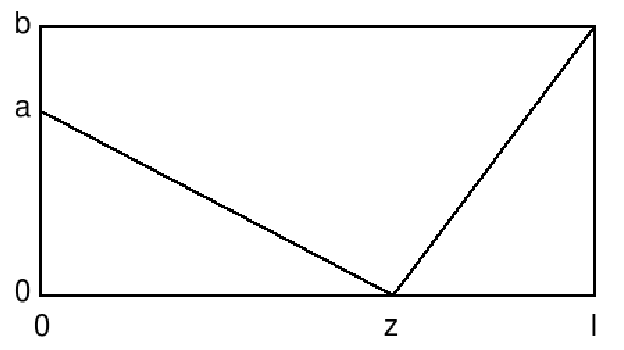
\includegraphics[width=2in]{trap}}
% este gráfico es cutre, se nota que es un jpg convertido. ¿No se puede
 % hacer mejor? - JJ
\caption{Generalised \emph{l-trap} function. }
\label{fig:trap}
\end{figure}
%%%%%%%%%%%%%%%%%%%%%%%%%%%%%%%%%%%


For the following experiments, 2-trap, 3-trap and 4-trap functions were designed with the following parameter values: $a = l-1$, $b = l$, and $z = l-1$. With these settings\footnote{Originally, Ackley's trap functions use $z=\frac{3l}{4}$, however, \cite{deb:deception} demonstrates that trap functions are fully easy under such settings.}, 2-trap  is not deceptive, 4-trap is deceptive and 3-trap lies in the region between deception and non-deception. Under these conditions, it is possible not only to examine the scalability on trap functions, but also to investigate how the scalability varies when changing from non-deceptive to deceptive search landscapes.
Scalability tests were performed by juxtaposing \textit{m}\ trap functions in binary strings of length $L$ and summing the fitness of each sub-function to obtain the total fitness. 


\subsection{A method for estimating the population size}
\label{sec:bisection}
%%%%%%%%%%%%%%%%%%%%%%%%%%%%%%%%%%%%%%%%%%%%%%%%%%%%%%%%%%%%%

Kumara Sastry proposes in \cite{sastry:bisection} a method based on bisection to  estimate
the optimal population size $N$ to solve a problem instance, that is, the lowest $N$ for which
98\% of the runs find the problem optimum. To this end, a selectorecombinative GA is used to search the minimum population size such that using random initialisation it is able to converge to the optimum without any other mechanism than recombination and selection. 

%%%%%%%%%%%%%%%%%%%%%%
\begin{algorithm}
\caption{Population tuning algorithm based on bisection}
\label{alg:bisection}
\begin{algorithmic}
\STATE $N$ = Initial Population Size ($20$)
\WHILE{ GA reliability ($N$) $<$ 98\%}
\STATE $min = N; max,N = 2N$
\ENDWHILE
\WHILE{ $\frac{max-min}{min} > \frac{1}{16}$}
\STATE $N = \frac{max+min}{2}$ 
\IF{ GA reliability($N$) $<$ 98\%}
\STATE $min = N$
\ELSE
\STATE $max = N$
\ENDIF
\ENDWHILE
\end{algorithmic}
\end{algorithm}
%%%%%%%%%%%%%%%%%%%%%%



Algorithm \ref{alg:bisection} depicts the method based on bisection.
The method begins with a small population size which is doubled until
the algorithm ensures a reliable convergence. We define the
reliability criterion as the convergence of the algorithm to the
optimum 49 out of 50 times. After that, the
interval $(\mathit{min},\mathit{max})$ is halved several times and the population size
adjusted within such a range until $\frac{\mathit{max}-\mathit{min}}{\mathit{min}} > \mathit{threshold}$,
where $\mathit{min}$ and $\mathit{max}$ stand respectively for the minimum and maximum population size estimated and $\mathit{threshold}$ for the accuracy of the adjustment within such a range. This parameter has been set to $\frac{1}{16}$ in order to obtain a good adjustment of the population size.




\subsection{Metrics}
\label{sec:metrics}
%%%%%%%%%%%%%%%%%%%%%%%%%%%%%%%%%%%%%%%%%%%%%%%%%%%%%%%%%%%%%

The following metrics \cite{eiben:eas} % Trata de cualificar siempre que
 % puedas las citas: as proposed by, as we have published in, as
 % reviewed by... tal como lo has puesto, no sé si es una descripción de
 % las métricas, una justificación de las mismas, o qué...
 will be used for assessing the performance of the model in the experimental analysis:

\begin{itemize}
\item The success rate (SR) measures the algorithm quality as the proportion in which the algorithm is able to find the problem optimum out of all the runs. 

\item The average number of evaluations to solution (AES) stands for the
      number of evaluations that the algorithm spends in those runs that
      yield success. Since a preliminary analysis on the normality of
      results shows that they do not follow a normal distribution, we
      have chosen the number of evaluations to solution in the third
      quartile ($AESQ_3$) as a central position value, meaning that a
      75\% of the runs will stay below such a value. % Third no es muy
      % central. Quizás es indicativo, pero central ni de coña.. - JJ

\item The Mean Best Fitness (MBF) is used to depict the algorithm convergence as the averaged values of the best fitness.

\item The genotypic entropy (GE) is a measure of the population diversity
  defined on the genotypic distances ($H_g(P)$). 

\begin{equation}
H_g(P)=-\sum_{j=1}^{N}{g_jlog(g_j)}
\end{equation}

\noindent where $g_j$ is the fraction $\frac{n_j}{N}$ of individuals in $P$ having a Hamming distance $j$ to the optimal genotype, and $N$ is the number of different distances.

\end{itemize}





%%%%%%%%%%%%%%%%%%%%%%%%%%%%%%%%%%%%%%%%%%%%%%%%%%%%%%%%%%%%%
\section{Conclusions}
\label{sec:methodolgyconclusions}
%%%%%%%%%%%%%%%%%%%%%%%%%%%%%%%%%%%%%%%%%%%%%%%%%%%%%%%%%%%%%

This chapter presents the experimental methodology that will be followed within the next chapter for analysing the viability of the EvAg approach. To that aim, we will have to prove that the algorithm is {\em scalable} and {\em fault-tolerant} in a simulated P2P environment.

In order to tackle such goals, we will perform an experimental analysis of the three test-cases summarised in Table \ref{table:methodology}. In every case, the analysis will follow the same methodology consisting in the study of the algorithmic scalability, the analysis of the algorithm convergence and population diversity at run-time and a comparison of the results to show whether they present statistical differences or not.

%La conclusión debe ser más fuerte, resumir más y preparar para el
%siguiente - JJ
\begin{sidewaystable}[htbp]
%\begin{table}[htbp]
\centering
{\scriptsize
\begin{tabular}{|c | c|}
\hline
Test-Case & Methodology \\
\hline
1 & 1.1 Scalability selectorecombinative GA\\
Scalability in a failure-free environment & 1.2 Analysis of the convergence of the larger problem instance\\
vs. sequential GAs& 1.3 Statistical analysis\\
\hline
2 & 2.1 Scalability selectorecombinative GA\\
Influence of the population structure & 2.2 Analysis of the convergence of the larger problem instance\\
on the algorithm performance & 2.3 Statistical analysis\\
\hline
3 & 3.1 Scalability selectorecombinative GA \\
Fault tolerance of the model & 3.2 Analysis of the convergence under different churn scenarios\\
& 3.3 Statistical analysis\\
\hline
\end{tabular}
}
\caption{Summary of the experimental methodology.\label{table:methodology}}
%\end{table}
\end{sidewaystable}


%%%%%%%%%%%%%% Bibliografia %%%%%%%%%%%%%%%

%\bibliographystyle{alpha}  % Eliminarlo al compilar el documento maestro, ponerlo para compilarlo separado
%\bibliography{pea,p2pcomputing,model,methodology}% Eliminarlo al compilar el documento maestro, ponerlo para compilarlo separado

%\end{document}             % Eliminarlo al compilar el documento maestro, ponerlo para compilarlo separado


%%%%%%%%%%%%%%%%%%%%%%%%%%%%%%%%%%%%%%%%%%%%%%%%%%%%%%%%%%%%%
%\sectio{Tunning of the Cache size parameter}
%\label{sec:tunningcache}
%%%%%%%%%%%%%%%%%%%%%%%%%%%%%%%%%%%%%%%%%%%%%%%%%%%%%%%%%%%%%

%This section explores the impact of different cache sizes on the algorithm performance given that cache size is the only tunable parameter in newscast.

%Table \ref{table:parameters} summarizes the settings of the experiments. Fourteen different cache sizes for the newscast protocol and two different population/network sizes\footnote{Population size referring to an EA is equivalent to network size in terms of a P2P system.} for the EA have been tested for every problem instance. The rest of the parameters are standard in EAs and a detailed explanation can be found in e.g. \cite{eiben:eas}.


%\begin{table}[htbp]
%\centering
%{\scriptsize
%\begin{tabular}{r c}
%\hline
%\multicolumn{2}{l}{\textbf{EA settings}}\\
%\hline
%EA type & Genetic Algorithm \\
%Proble instance & 3-Trap\\
%Population size 3-Trap & 480, 240 individuals \\
%Recombination & Uniform Crossover, $p_c = 1.0$ \\
%Selection Parents & Binary Tournament \\
%\hline
%\multicolumn{2}{l}{\textbf{Newscast settings}}\\
%\hline
% $Cache_{size}$ & 8, 16,24,32,48,64,128\\
%\hline
%\end{tabular}
%}
%\caption{Parameters of the algorithms\label{table:parameters}}
%\end{table}





%%%%%%%%%%%%%%%%%%%%%%%%%%%%%%%%%%%%%%%%%%%%%%%%%%%%%%%%%%%%%%
%\begin{table*}[htbp]
%\centering
%{\tiny
%\begin{tabular}{|r|c c c c c c c ||c c c c c c c |}
%\hline
%&\multicolumn{7}{|c||}{p-value}&\multicolumn{7}{c|}{Significantly different?}\\
%\hline
%& 8 & 16 & 24 & 32 & 48 & 64 & 128 & 8 & 16 & 24 & 32 & 48 & 64 & 128 \\
%\hline
%8  & x   & 0.003  & 0.00008  & 0.00004  & 0.00005  & 0.000008  & 0.0001  & x & + & + & + & + & + & + \\
%16 & 0.92  & x   & 0.73  & 0.72  & 0.30  & 0.19  & 0.32  & - & x & - & - & - & - & - \\
%24 & 0.25  & 0.16  & x   & 0.89  & 0.52  & 0.24  & 0.50  & - & - & x & - & - & - & - \\
%32 & 0.91  & 0.85  & 0.15  & x   & 0.55  & 0.39  & 0.55  & - & - & - & x & - & - & - \\
%48 & 0.55  & 0.36  & 0.48  & 0.64  & x   & 0.72  & 0.97  & - & - & - & - & x & - & - \\
%64 & 0.31  & 0.16  & 0.84  & 0.19  & 0.58  & x   & 0.73  & - & - & - & - & - & x & - \\
%128& 0.21  & 0.18  & 1  & 0.09  & 0.46  & 0.85  & x   & - & - & - & - & - & - & x \\
%\hline
%\end{tabular}
%}
%\caption{Population size 480 (superior) 240 (inferior)
%\label{table:cachesizes}}
%\end{table*}
%%%%%%%%%%%%%%%%%%%%%%%%%%%%%%%%%%%%%%%%%%%%%%%%%%%%%%%%%%%%%%

%%%%%%%%%%%%%%%%%%%%%%%%%%%%%%%%%%%%%%%%%%%%%%%%%%%%%%%%%%%%%%
%\begin{table*}[htbp]
%\centering
%{\tiny
%\begin{tabular}{|r|c c c c c c c|}
%\hline
%$N=480$&\multicolumn{7}{c|}{Significantly different?}\\
%\hline
%Cache sizes ($c$)& 8 & 16 & 24 & 32 & 48 & 64 & 128 \\
%\hline
%8 & x & yes & yes & yes & yes & yes & yes \\
%16 & yes & x & no & no & no & no & no \\
%24 & yes & no & x & no & no & no & no \\
%32 & yes & no & no & x & no & no & no \\
%48 & yes & no & no & no & x & no & no \\
%64 & yes & no & no & no & no & x & no \\
%128 & yes & no & no & no & no & no & x \\
%\hline
%\end{tabular}
%}
%\caption{Population size 480 (superior) 240 (inferior)
%\label{table:cachesizes}}
%\end{table*}
%%%%%%%%%%%%%%%%%%%%%%%%%%%%%%%%%%%%%%%%%%%%%%%%%%%%%%%%%%%%%%

%%%%%%%%%%%%%%%%%%%%%%%%%%%%%%%%%%%%%%%%%%%%%%%%%%%%%%%%%%%%%%
%\begin{table*}[htbp]
%\centering
%{\tiny
%\begin{tabular}{|r|c c c c c c c|}
%\hline
%$N=240$&\multicolumn{7}{c|}{Significantly different?}\\
%\hline
%Cache sizes ($c$)& 8 & 16 & 24 & 32 & 48 & 64 & 128 \\
%\hline
%8 & x & no & no & no & no & no & no \\
%16 & no & x & no & no & no & no & no \\
%24 & no & no & x & no & no & no & no \\
%32 & no & no & no & x & no & no & no \\
%48 & no & no & no & no & x & no & no \\
%64 & no & no & no & no & no & x & no \\
%128 & no & no & no & no & no & no & x \\
%\hline
%\end{tabular}
%}
%\caption{Population size 480 (superior) 240 (inferior)
%\label{table:cachesizes}}
%\end{table*}
%%%%%%%%%%%%%%%%%%%%%%%%%%%%%%%%%%%%%%%%%%%%%%%%%%%%%%%%%%%%%%




%\begin{figure}[htbp]
%\centerline{
%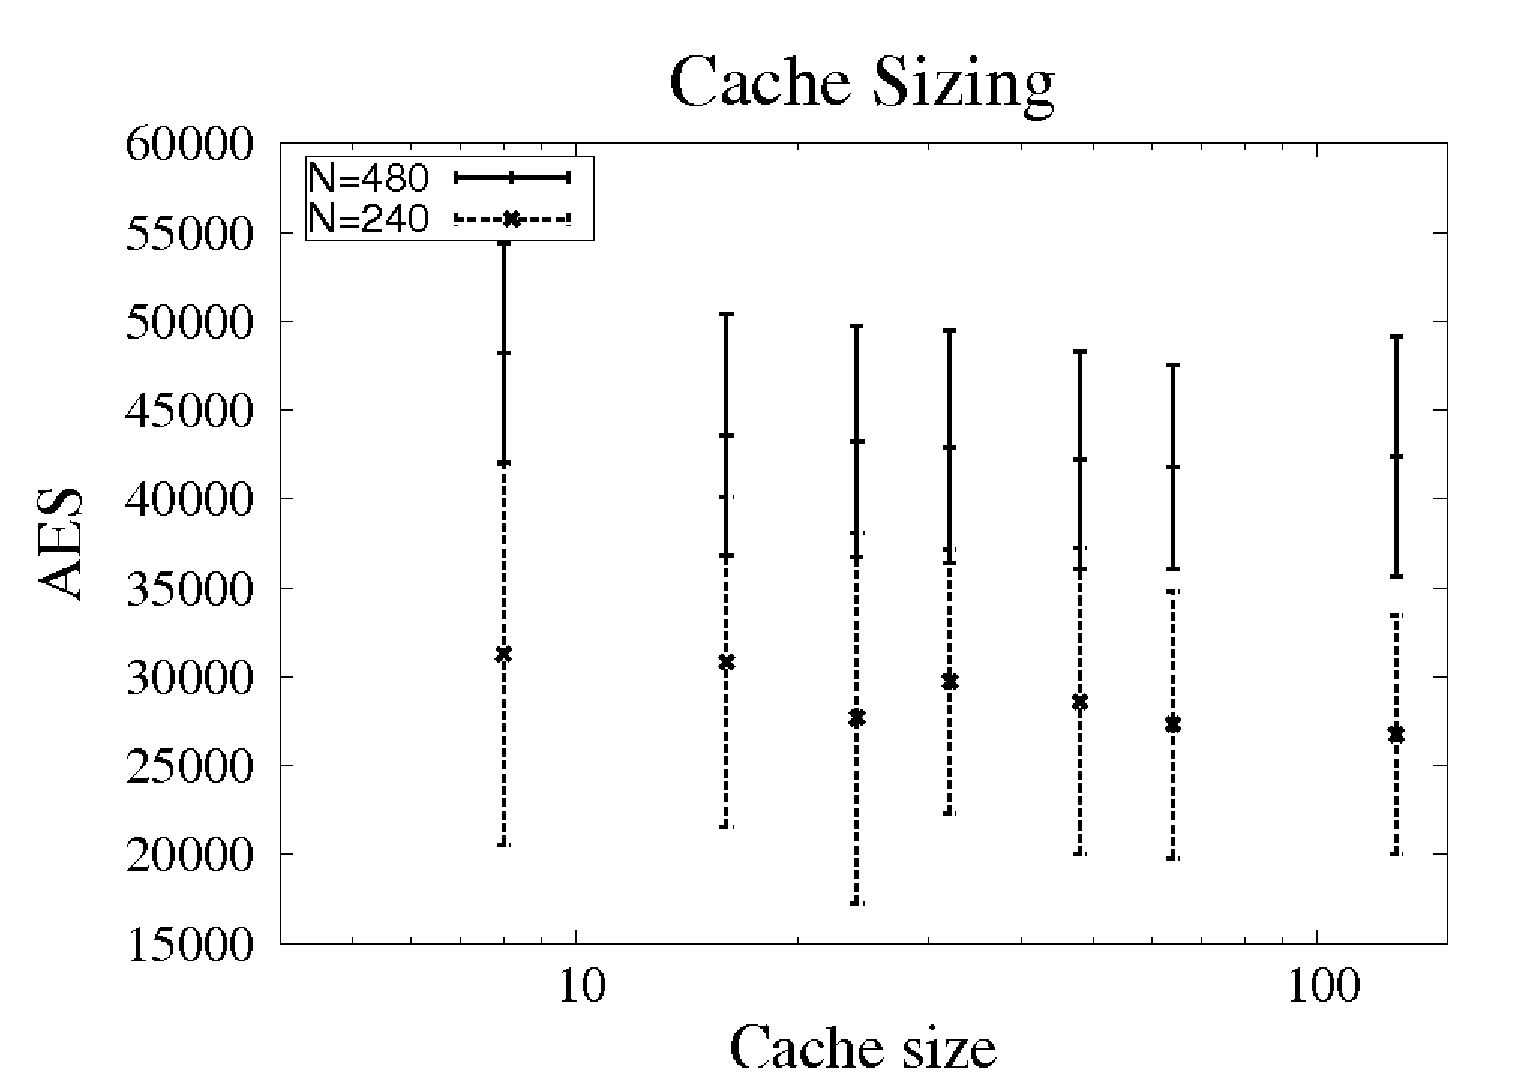
\includegraphics[width=0.6\textwidth]{aescache}
%}
%\caption{Average Evaluation to Solution with standard deviation of the EvAg model for different cache sizes in a 3-Trap instance. Population/network sizes of $N=240$ and $N=480$.}
%\label{fig:aescache}
%\end{figure}

%Figures \ref{fig:mmdp}  and \ref{fig:wppeak} show the SR and AES of the EvAg 
%model when tackling the 3-Trap instance for different cache and network sizes. In both cases, it can be observed that the network size impacts on the algorithm performance while the cache size does not. Larger network sizes improve the quality of the solutions but increase the computational effort. However, considering different cache sizes, the algorithm does not change either in terms of quality (SR) or run-time (AES).  


%Results on the 3-Trap instance show that the algorithm quality and run-time are not altered when changing the settings of the cache size. This fact translates into the robustness of the EvAg model with respect to the cache size parameter and is specially remarkable from the point of view of tuning the algorithm parameters.

%Results in the two different instances can be analysed as follows:

%MMDP: The algorithm converges with a SR around 0.9 using a network size of $N=440$. For $N=200$ the SR decreases to $\sim$0.2 showing that the P2P EA  is quite sensitive to the network size when tackling the MMDP. Regarding cache sizes, results around the same averaged quality and run-time show the independence of the algorithm performance with respect to such a parameter. Additionally, there is not a clear trend toward the way the performances vary when changing the cache size values and variations around the average can be explained as an stochastic effect of EAs.

%\begin{figure}[htbp]
%\centerline{
%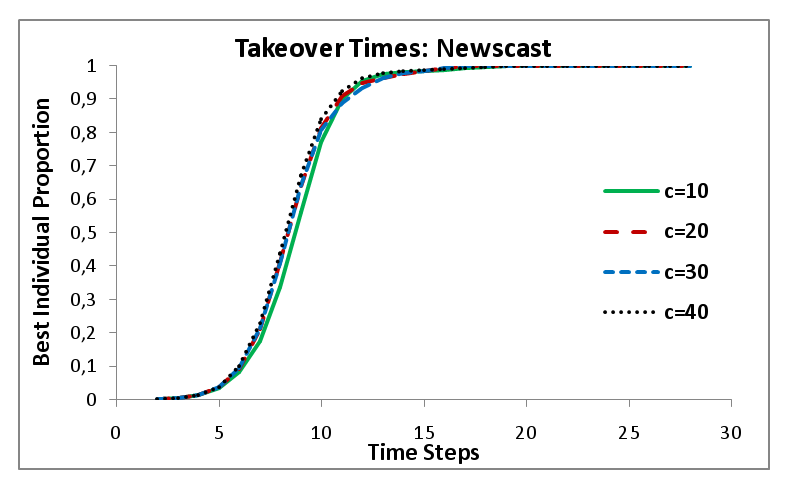
\includegraphics[width=0.6\textwidth]{takeovercache}
%}
%\caption{Takeover Times curves}
%\label{fig:takeovercache}
%\end{figure}

